\documentclass[a4paper]{article}
\usepackage{amsfonts}
\usepackage{amsmath}
\usepackage{amssymb}
\usepackage{graphicx}

\begin{document}
  
\noindent \large Auteur: Thijs Van Schel \\
\noindent \large Studierichting: Informatica\\
\noindent \large Oefeningenreeks 5J nr. 2.1\\

\medskip

$L = \displaystyle\int\limits_0^{2\pi}\sqrt{(x'(t))^2+(y'(t))^2}dt$\\

$x'(t) = a(1-\cos(t)$\\

$y'(t) = a(0+\sin(t)) = a\sin(t))$\\

$\Rightarrow \displaystyle\int\limits_0^{2\pi} a\sqrt{(1-\cos(t))^2+(\sin(t))^2} dt$\\

$ = \displaystyle\int\limits_0^{2\pi} a\sqrt{1-2\cos(t)+(\cos^2(t)+\sin^2(t))} dt$\\

$ = \displaystyle\int\limits_0^{2\pi} a\sqrt{1-2\cos(t)}dt$\\

$ = \displaystyle\int\limits_0^{2\pi} a\sqrt{2(1-\cos(t)}dt$\\

$ = a\sqrt{2}\displaystyle\int\limits_0^{2\pi} \sqrt{1-\cos(t)}dt$\\

verdubbeling hoek: $ \cos(t) = 1 - 2\sin^2\left(\dfrac{t}{2}\right)$\\

$ = a\sqrt{2}\displaystyle\int\limits_0^{2\pi} \sqrt{1-1+2\sin^2\dfrac{t}{2}}dt$\\

$ = a\sqrt{2}\displaystyle\int\limits_0^{2\pi} \sqrt{2\sin^2\dfrac{t}{2}}dt$\\

$ = a\sqrt{2}\displaystyle\int\limits_0^{2\pi} \sqrt{2}\sin\dfrac{t}{2}dt$\\

$ = 2a\displaystyle\int\limits_0^{2\pi} \sin\dfrac{t}{2}dt$\\

$ = 4a \left[-\cos\left(\dfrac{t}{2}\right)\right]^{2\pi}_0$\\

$ = 4a(-\cos\pi + \cos0) = 8a$
\normalsize

\begin{figure}[h]
    \centering
    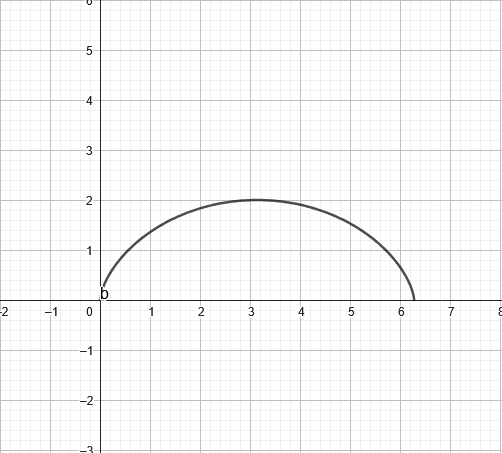
\includegraphics[width=0.6\textwidth]{5J-2.1-thijs.van.schel.INF.png}
\end{figure}

\begin{thebibliography}{999}
%\bibitem{a} Referentie
\end{thebibliography}
\end{document} 
